\documentclass[11pt]{article}
\usepackage[margin=2.5cm]{geometry}
\usepackage{booktabs}
\usepackage{graphicx}
\usepackage{caption}
\usepackage{subcaption}
\usepackage{wrapfig}
\usepackage{fancyhdr}
\usepackage{amsmath}
\usepackage{amssymb}

\title{\textbf{Large Subway Systems as Complex Networks}}
\author{Panagiotis Angeloudis, David Fisk}

\begin{document}
\maketitle

\begin{center}
\textbf{Summarised by Ryan Stickland}
\end{center}

This paper presents a study of modern large city underground subway systems and constructs them as complex networks. 20 of the world’s larges subway systems from across the world were analysed and the properties of such networks evaluated. As well as this they constructed their own model of a ‘toy subway’, which was a subway network they grew computationally using methods they approximated as the way subway systems grow in the real world.\\

They started by analysing the common characteristics of world subway networks. These include typical aspects such as degree distribution and mean shortest path. They found these values aren’t representative of traditional small-world or scale-free networks, this is to be expected due to the fact that subways usually grow not by addition of single nodes but by long chains of nodes and edges i.e. new lines. Figure 1 shows the degree distribution their subways. Unsurprisingly, there are many stations with degree 2 i.e. through stations.\\

They started by analysing the common characteristics of world subway networks. These include typical aspects such as degree distribution and mean shortest path. They found these values aren’t representative of traditional small-world or scale-free networks, this is to be expected due to the fact that subways usually grow not by addition of single nodes but by long chains of nodes and edges i.e. new lines. Figure 1 shows the degree distribution their subways. Unsurprisingly, there are many stations with degree 2 i.e. through stations.\\

They then created their model for subway growth. They added long chains of nodes (lines), one at a time, and calculated the subsequent degree distribution. They derived a recursive relationship for degree distribution and a formulation for the probability of a new station being connected to an existing station. From this they concluded that their model for subway systems obey an exponential degree distribution. Figure 2 shows a log plot of their degree distribution (black line) compare with those of worldwide subway systems. It seems as though their model is a very good fit for most systems. There is a cluster of outliers, which they say mainly come from German. This not surprising to them as many subway systems there are based on old tram lines which share track (edges) between lines.\\

They then reviewed global subway systems’ resilience against random and targeted attacks. They found that, due to the exponential degree distribution, networks are very resilient against random attacks (due to the low degree of most stations). They are however also quite resilient to targeted attacks on high degree-stations and (tragically) have real-world evidence to back that claim up in the form of Madrid 2004 and London 2005 subway attacks.\\

Complex networks are an extremely useful concept in statistical mechanics. Many statistical systems e.g. ensembles, collections of particles and quantum states etc. can be modelled as complex networks, with interactions between them considered as edges. Concepts discussed here such as degree distributions and mean shortest path are useful in determining properties of statistical systems such as entropy, temperature and other concerned observables. Subway systems are a type of complex network that arise 'naturally' in our world due to physical constraints, so study of these can teach us about how to apply these concepts to other types of networks that may be more difficult to physically measure.

\begin{figure}[h]
	\begin{subfigure}{0.5\textwidth}
		\centering
		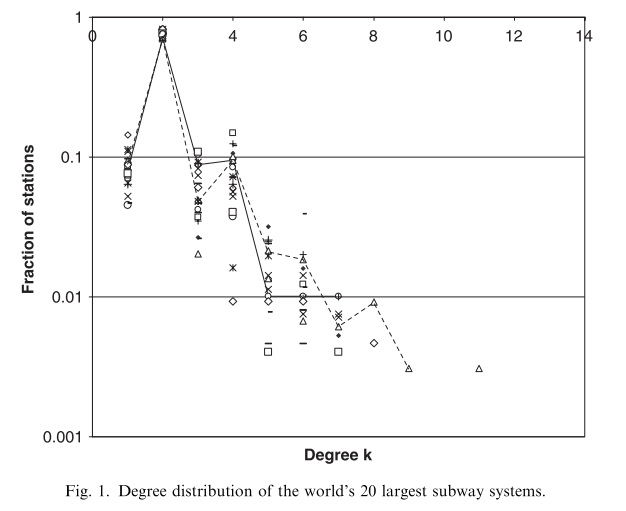
\includegraphics[scale=1]{Stickland_q3_fig1.png}
	\end{subfigure}
	\begin{subfigure}{0.5\textwidth}
		\centering
		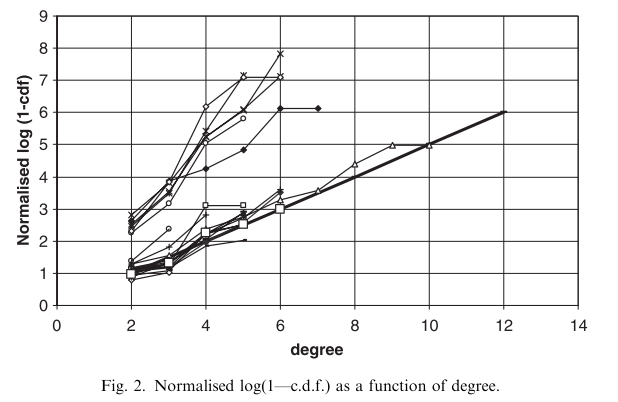
\includegraphics[scale=1]{Stickland_q3_fig2.png}
	\end{subfigure}
\end{figure}

\end{document}